\documentclass[twoside]{book}

% Packages required by doxygen
\usepackage{fixltx2e}
\usepackage{calc}
\usepackage{doxygen}
\usepackage[export]{adjustbox} % also loads graphicx
\usepackage{graphicx}
\usepackage[utf8]{inputenc}
\usepackage{makeidx}
\usepackage{multicol}
\usepackage{multirow}
\PassOptionsToPackage{warn}{textcomp}
\usepackage{textcomp}
\usepackage[nointegrals]{wasysym}
\usepackage[table]{xcolor}

% Font selection
\usepackage[T1]{fontenc}
\usepackage[scaled=.90]{helvet}
\usepackage{courier}
\usepackage{amssymb}
\usepackage{sectsty}
\renewcommand{\familydefault}{\sfdefault}
\allsectionsfont{%
  \fontseries{bc}\selectfont%
  \color{darkgray}%
}
\renewcommand{\DoxyLabelFont}{%
  \fontseries{bc}\selectfont%
  \color{darkgray}%
}
\newcommand{\+}{\discretionary{\mbox{\scriptsize$\hookleftarrow$}}{}{}}

% Page & text layout
\usepackage{geometry}
\geometry{%
  a4paper,%
  top=2.5cm,%
  bottom=2.5cm,%
  left=2.5cm,%
  right=2.5cm%
}
\tolerance=750
\hfuzz=15pt
\hbadness=750
\setlength{\emergencystretch}{15pt}
\setlength{\parindent}{0cm}
\setlength{\parskip}{0.2cm}
\makeatletter
\renewcommand{\paragraph}{%
  \@startsection{paragraph}{4}{0ex}{-1.0ex}{1.0ex}{%
    \normalfont\normalsize\bfseries\SS@parafont%
  }%
}
\renewcommand{\subparagraph}{%
  \@startsection{subparagraph}{5}{0ex}{-1.0ex}{1.0ex}{%
    \normalfont\normalsize\bfseries\SS@subparafont%
  }%
}
\makeatother

% Headers & footers
\usepackage{fancyhdr}
\pagestyle{fancyplain}
\fancyhead[LE]{\fancyplain{}{\bfseries\thepage}}
\fancyhead[CE]{\fancyplain{}{}}
\fancyhead[RE]{\fancyplain{}{\bfseries\leftmark}}
\fancyhead[LO]{\fancyplain{}{\bfseries\rightmark}}
\fancyhead[CO]{\fancyplain{}{}}
\fancyhead[RO]{\fancyplain{}{\bfseries\thepage}}
\fancyfoot[LE]{\fancyplain{}{}}
\fancyfoot[CE]{\fancyplain{}{}}
\fancyfoot[RE]{\fancyplain{}{\bfseries\scriptsize Generated on Fri Jul 24 2015 13\+:15\+:26 for L\+L\+V\+M Data Flow Graphs by Doxygen }}
\fancyfoot[LO]{\fancyplain{}{\bfseries\scriptsize Generated on Fri Jul 24 2015 13\+:15\+:26 for L\+L\+V\+M Data Flow Graphs by Doxygen }}
\fancyfoot[CO]{\fancyplain{}{}}
\fancyfoot[RO]{\fancyplain{}{}}
\renewcommand{\footrulewidth}{0.4pt}
\renewcommand{\chaptermark}[1]{%
  \markboth{#1}{}%
}
\renewcommand{\sectionmark}[1]{%
  \markright{\thesection\ #1}%
}

% Indices & bibliography
\usepackage{natbib}
\usepackage[titles]{tocloft}
\setcounter{tocdepth}{3}
\setcounter{secnumdepth}{5}
\makeindex

% Hyperlinks (required, but should be loaded last)
\usepackage{ifpdf}
\ifpdf
  \usepackage[pdftex,pagebackref=true]{hyperref}
\else
  \usepackage[ps2pdf,pagebackref=true]{hyperref}
\fi
\hypersetup{%
  colorlinks=true,%
  linkcolor=blue,%
  citecolor=blue,%
  unicode%
}

% Custom commands
\newcommand{\clearemptydoublepage}{%
  \newpage{\pagestyle{empty}\cleardoublepage}%
}


%===== C O N T E N T S =====

\begin{document}

% Titlepage & ToC
\hypersetup{pageanchor=false,
             bookmarks=true,
             bookmarksnumbered=true,
             pdfencoding=unicode
            }
\pagenumbering{roman}
\begin{titlepage}
\vspace*{7cm}
\begin{center}%
{\Large L\+L\+V\+M Data Flow Graphs \\[1ex]\large 0.\+1 }\\
\vspace*{1cm}
{\large Generated by Doxygen 1.8.9.1}\\
\vspace*{0.5cm}
{\small Fri Jul 24 2015 13:15:26}\\
\end{center}
\end{titlepage}
\clearemptydoublepage
\tableofcontents
\clearemptydoublepage
\pagenumbering{arabic}
\hypersetup{pageanchor=true}

%--- Begin generated contents ---
\chapter{Main Page}
\label{index}\hypertarget{index}{}\href{https://circleci.com/gh/k3ut0i/llvm-dataflow-graphs}{\tt !\mbox{[}Build\mbox{]}(https\+://circleci.\+com/gh/k3ut0i/xmonad-\/conf.\+svg?style=shield\&circle-\/token=\+:circle-\/token)}

This is similar to graph-\/llvm-\/ir by pfalcon. but there seems to be some problems for it.

Current Status\+:
\begin{DoxyEnumerate}
\item Control flow is good per function. should add?? between function blocks and calling statements??.
\item Data flow just getting started. It\textquotesingle{}s sample test code. ```c 
\begin{DoxyCode}
\textcolor{preprocessor}{#include <stdio.h>}
\textcolor{comment}{/*\{\{\{*/}
\textcolor{keywordtype}{int} f0(\textcolor{keywordtype}{int} x0 , \textcolor{keywordtype}{int} x6)\{
    \textcolor{keywordtype}{int} ans = 0;
    ans += (x0>x6)? x0: x6;
    \textcolor{keywordflow}{return} ans;
\}
\textcolor{comment}{/*\}\}\}*/}
\textcolor{keywordtype}{int} piped\_x0, piped\_x1;

\textcolor{keywordtype}{int} main()
\{
    piped\_x0 = 0;
    piped\_x1 = 1;
    printf(\textcolor{stringliteral}{"%d\(\backslash\)n"}, f0(piped\_x0, piped\_x1));
\}
\end{DoxyCode}
 ```c
\end{DoxyEnumerate}

Output Dot image  
\chapter{Namespace Index}
\section{Namespace List}
Here is a list of all documented namespaces with brief descriptions\+:\begin{DoxyCompactList}
\item\contentsline{section}{\hyperlink{namespacellvmutils}{llvmutils} }{\pageref{namespacellvmutils}}{}
\end{DoxyCompactList}

\chapter{Hierarchical Index}
\section{Class Hierarchy}
This inheritance list is sorted roughly, but not completely, alphabetically\+:\begin{DoxyCompactList}
\item Module\+Pass\begin{DoxyCompactList}
\item \contentsline{section}{datautils\+:\+:Data\+Worker}{\pageref{structdatautils_1_1DataWorker}}{}
\end{DoxyCompactList}
\end{DoxyCompactList}

\chapter{Class Index}
\section{Class List}
Here are the classes, structs, unions and interfaces with brief descriptions\+:\begin{DoxyCompactList}
\item\contentsline{section}{\hyperlink{structdatautils_1_1DataWorker}{datautils\+::\+Data\+Worker} }{\pageref{structdatautils_1_1DataWorker}}{}
\end{DoxyCompactList}

\chapter{Namespace Documentation}
\hypertarget{namespacellvmutils}{}\section{llvmutils Namespace Reference}
\label{namespacellvmutils}\index{llvmutils@{llvmutils}}
\subsection*{Functions}
\begin{DoxyCompactItemize}
\item 
\hypertarget{namespacellvmutils_a6e5b5c0df2940f93b257c942f7a6ff97}{}std\+::string {\bfseries L\+L\+V\+M\+Type\+As\+String} (const llvm\+::\+Type $\ast$T)\label{namespacellvmutils_a6e5b5c0df2940f93b257c942f7a6ff97}

\item 
\hypertarget{namespacellvmutils_a0d3766e22426ecedfe01de99ac00b7d6}{}std\+::string {\bfseries L\+L\+V\+M\+Instruction\+As\+String} (llvm\+::\+Instruction $\ast$I)\label{namespacellvmutils_a0d3766e22426ecedfe01de99ac00b7d6}

\end{DoxyCompactItemize}


\subsection{Detailed Description}
The implementqation of llvmtypeasstring fucntion was copied from some code which i don\textquotesingle{}t remember tell me if anyone cares. 
\chapter{Class Documentation}
\hypertarget{structdatautils_1_1DataWorker}{}\section{datautils\+:\+:Data\+Worker Struct Reference}
\label{structdatautils_1_1DataWorker}\index{datautils\+::\+Data\+Worker@{datautils\+::\+Data\+Worker}}
Inheritance diagram for datautils\+:\+:Data\+Worker\+:\begin{figure}[H]
\begin{center}
\leavevmode
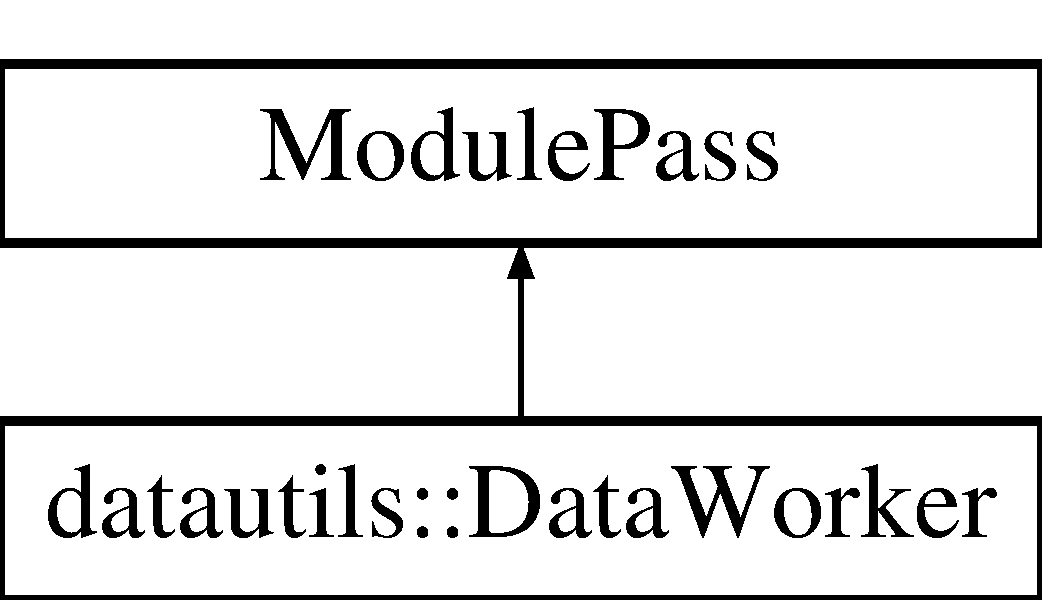
\includegraphics[height=2.000000cm]{structdatautils_1_1DataWorker}
\end{center}
\end{figure}
\subsection*{Public Member Functions}
\begin{DoxyCompactItemize}
\item 
\hypertarget{structdatautils_1_1DataWorker_ac2b68d9511a0c012c2575dc2bbbe2d15}{}bool {\bfseries run\+On\+Module} (llvm\+::\+Module \&M)\label{structdatautils_1_1DataWorker_ac2b68d9511a0c012c2575dc2bbbe2d15}

\end{DoxyCompactItemize}
\subsection*{Static Public Attributes}
\begin{DoxyCompactItemize}
\item 
\hypertarget{structdatautils_1_1DataWorker_ab2791f26c5f06a2d45ce48df4656467b}{}static char {\bfseries I\+D} = 0\label{structdatautils_1_1DataWorker_ab2791f26c5f06a2d45ce48df4656467b}

\end{DoxyCompactItemize}


\subsection{Detailed Description}


Definition at line 18 of file dataflow.\+h.



The documentation for this struct was generated from the following files\+:\begin{DoxyCompactItemize}
\item 
dataflow.\+h\item 
dataflow.\+cc\end{DoxyCompactItemize}

%--- End generated contents ---

% Index
\backmatter
\newpage
\phantomsection
\clearemptydoublepage
\addcontentsline{toc}{chapter}{Index}
\printindex

\end{document}
